\documentclass[12pt]{article}

\usepackage[margin=1in]{geometry}
\usepackage{graphicx}
\usepackage{amsmath}
\usepackage{booktabs}
\usepackage{hyperref}
\usepackage{float}
\usepackage{caption}
\usepackage{subcaption}

\title{Modeling Complex Contagion in a Discord Community Using Knowledge Graphs}
\author{Riley Sinema \\ CS 575 -- Graph Data Science}
\date{\today}

\begin{document}

\maketitle

\begin{abstract}
This report analyzes a Discord server used by an undergraduate CS course to model how beneficial academic behaviors might spread among students. I construct a knowledge graph from anonymized interaction data, project it into a user-user network, and apply centrality measures and community detection to identify influential nodes. The network exhibits a dense core-periphery structure rather than well-separated communities, with a small number of TAs and highly active students occupying central positions across all metrics. These findings inform early adopter selection strategies for a fractional threshold complex contagion model, with the goal of maximizing behavior adoption through targeted interventions.
\end{abstract}

% =============================================================================
\section{Introduction}
% =============================================================================

Encouraging students to adopt productive academic behaviors -- such as writing tests before coding, reading material before class, or reviewing peers' code -- is a persistent challenge in CS education. These behaviors are not adopted in isolation; they spread through social reinforcement, where a student is more likely to adopt a behavior when multiple peers have already done so. This makes them a natural fit for \textit{complex contagion} models, which require exposure from multiple sources before adoption occurs.

This project uses interaction data from a Discord server associated with an undergraduate CS course. I construct a knowledge graph capturing students, TAs, threads, and channels, then project it onto a user-user network to analyze the social structure underlying the course community. Using centrality metrics, community detection, and complex contagion simulation, I identify which individuals and structures are most important for maximizing the spread of desirable behaviors.

% =============================================================================
\section{Knowledge Graph Construction}
% =============================================================================

\subsection{Dataset and Graph Schema}

The dataset consists of two CSV files (\texttt{nodes.csv} and \texttt{edges.csv}) describing entities and interactions in a Discord server. The knowledge graph contains three node types:

\begin{itemize}
    \item \textbf{Person} -- students, TAs, and instructors (315 nodes)
    \item \textbf{Thread} -- discussion threads within channels (342 nodes)
    \item \textbf{Channel} -- Discord channels (14 nodes)
\end{itemize}

Each person node carries a \texttt{node\_value} attribute indicating their role (Student, TA, or Instructor). Edges represent interactions: replies between users, thread participation, message authorship, and channel membership. The full graph contains 671 nodes and 1{,}859 edges.

\begin{figure}[H]
    \centering
    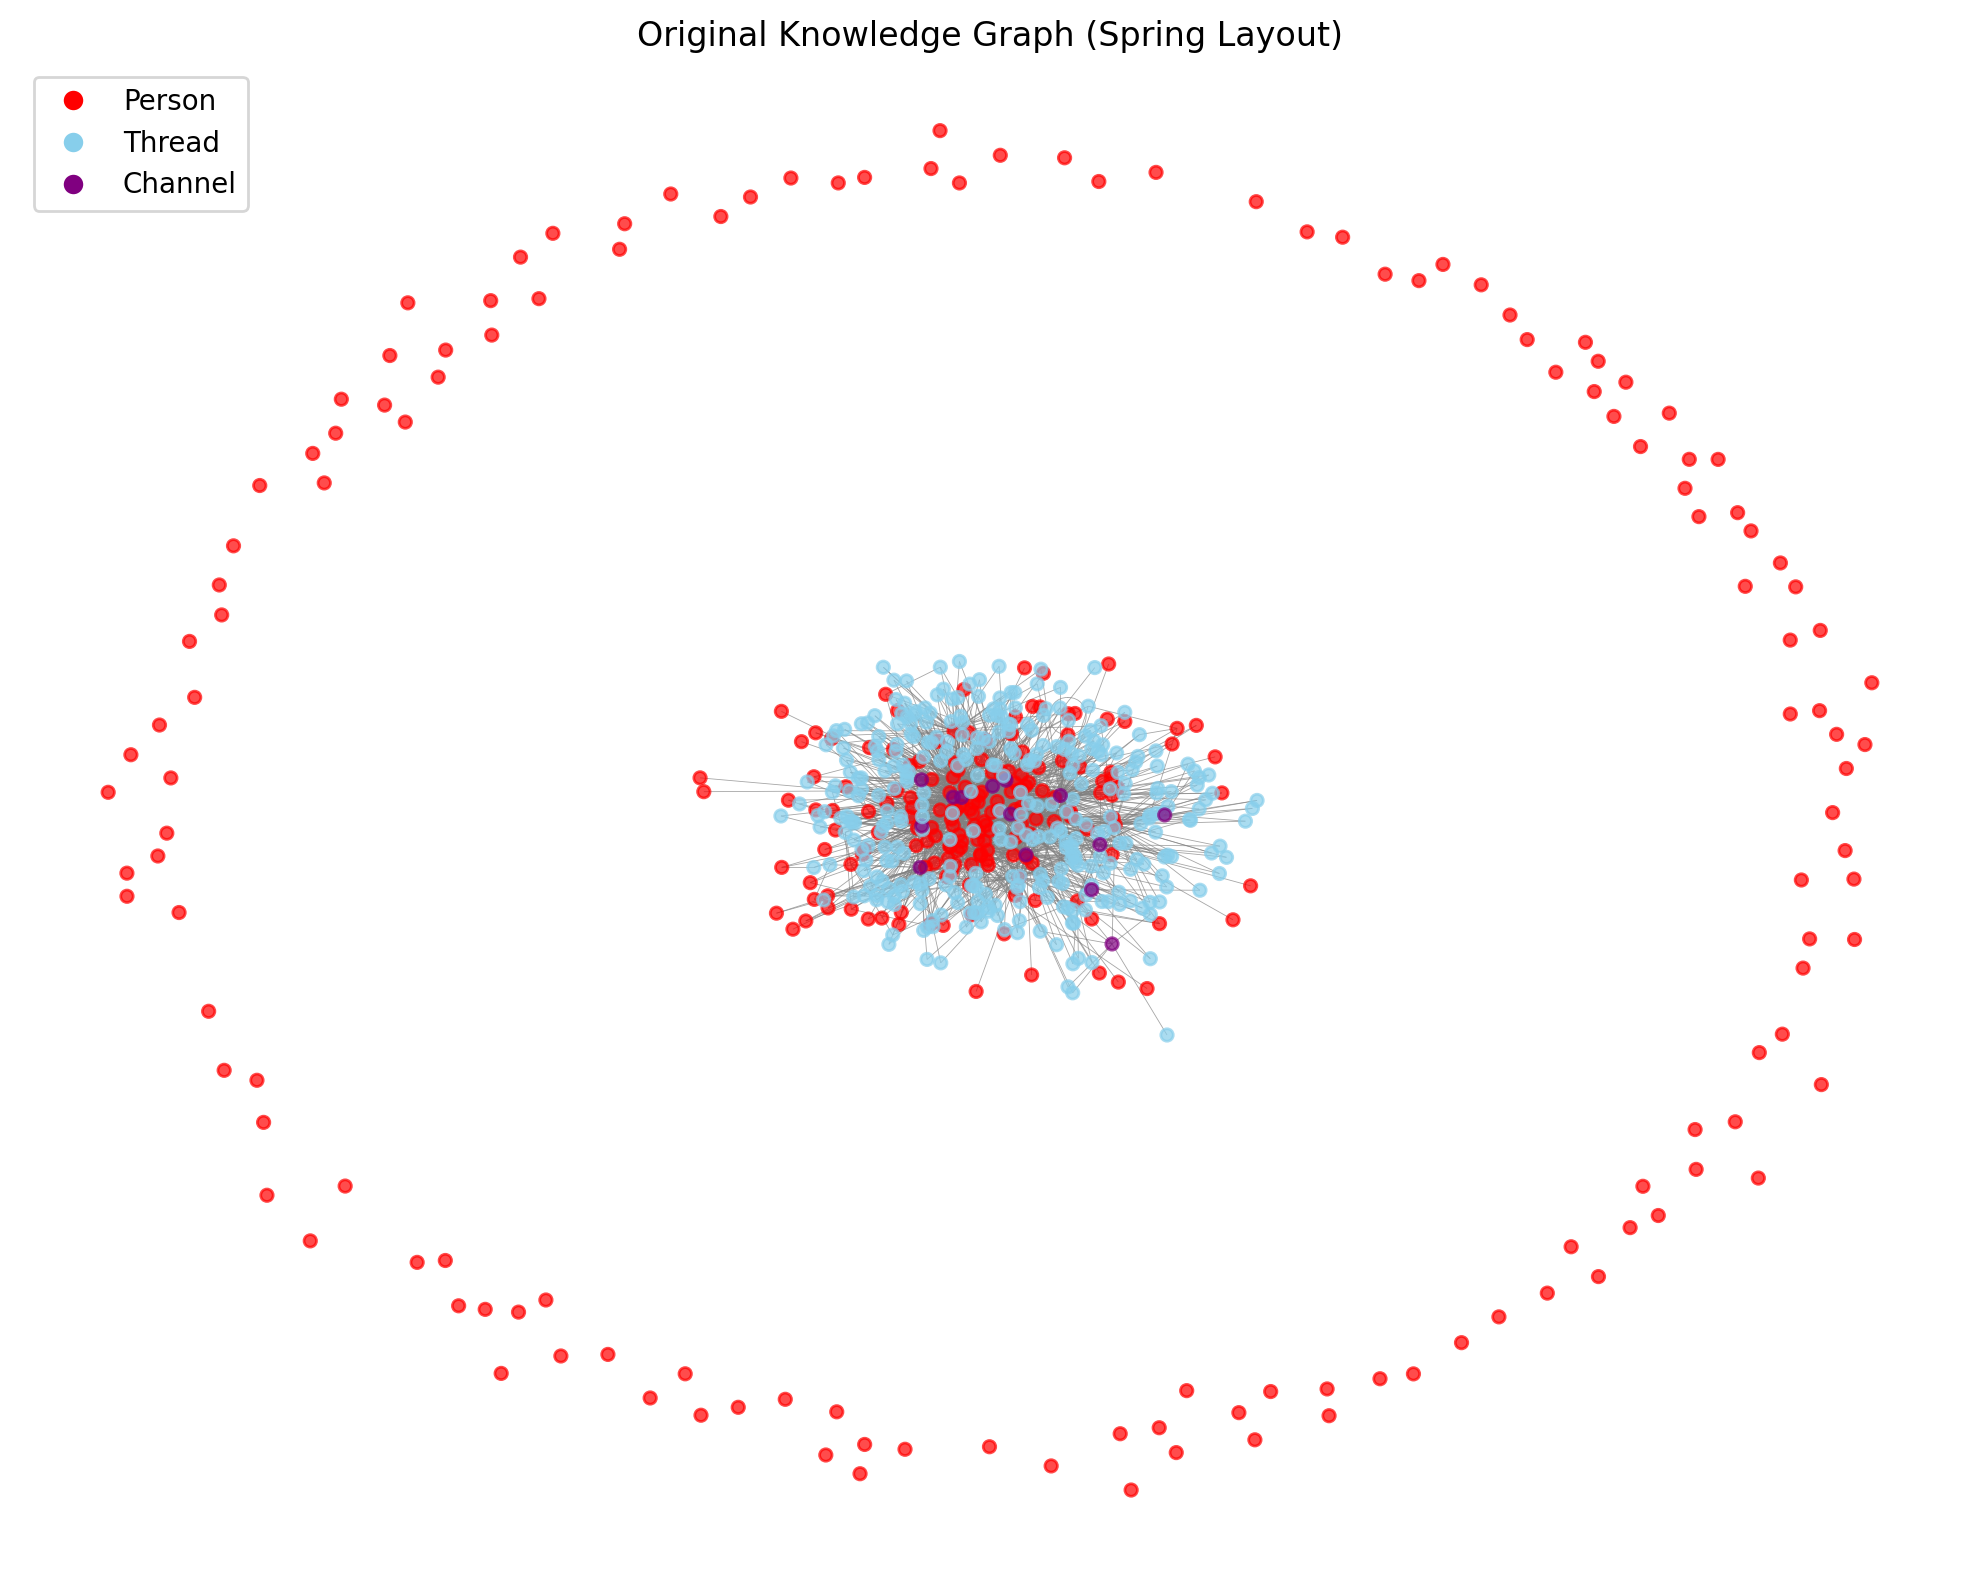
\includegraphics[width=0.85\textwidth]{figs/original_graph.png}
    \caption{The original knowledge graph visualized with a spring layout. Red nodes are persons, blue nodes are threads, and purple nodes are channels.}
    \label{fig:original_graph}
\end{figure}

\subsection{Loading the Graph}

The graph was provided as a GraphML file and loaded into NetworkX using \texttt{nx.read\_graphml()}. Basic inspection confirmed the expected node type distribution: 315 persons, 342 threads, and 14 channels.

\subsection{One-Mode Projection}

The original knowledge graph is heterogeneous, containing multiple node types. To analyze person-to-person social structure, I apply a one-mode projection that collapses the bipartite relationships into a single user-user network.

For each pair of node types (person-thread, person-channel), I construct a biadjacency matrix $B$ where $B_{ij} = 1$ if person $i$ is connected to entity $j$. The one-mode projection is computed as $P = B \cdot B^T$, where entry $P_{ij}$ counts the number of shared entities between persons $i$ and $j$. I also include direct person-to-person edges (e.g., replies). The three projection matrices are summed to produce a combined co-participation matrix, and any pair with a nonzero entry is connected in the projected graph.

The resulting projected graph contains all 315 person nodes and 8{,}704 edges. However, 141 of these nodes are isolates (persons with no shared threads, channels, or direct interactions with other persons). Removing isolates yields a connected graph of 174 nodes (163 students, 10 TAs, 1 instructor) and 8{,}704 edges.

\begin{figure}[H]
    \centering
    \begin{subfigure}[b]{0.48\textwidth}
        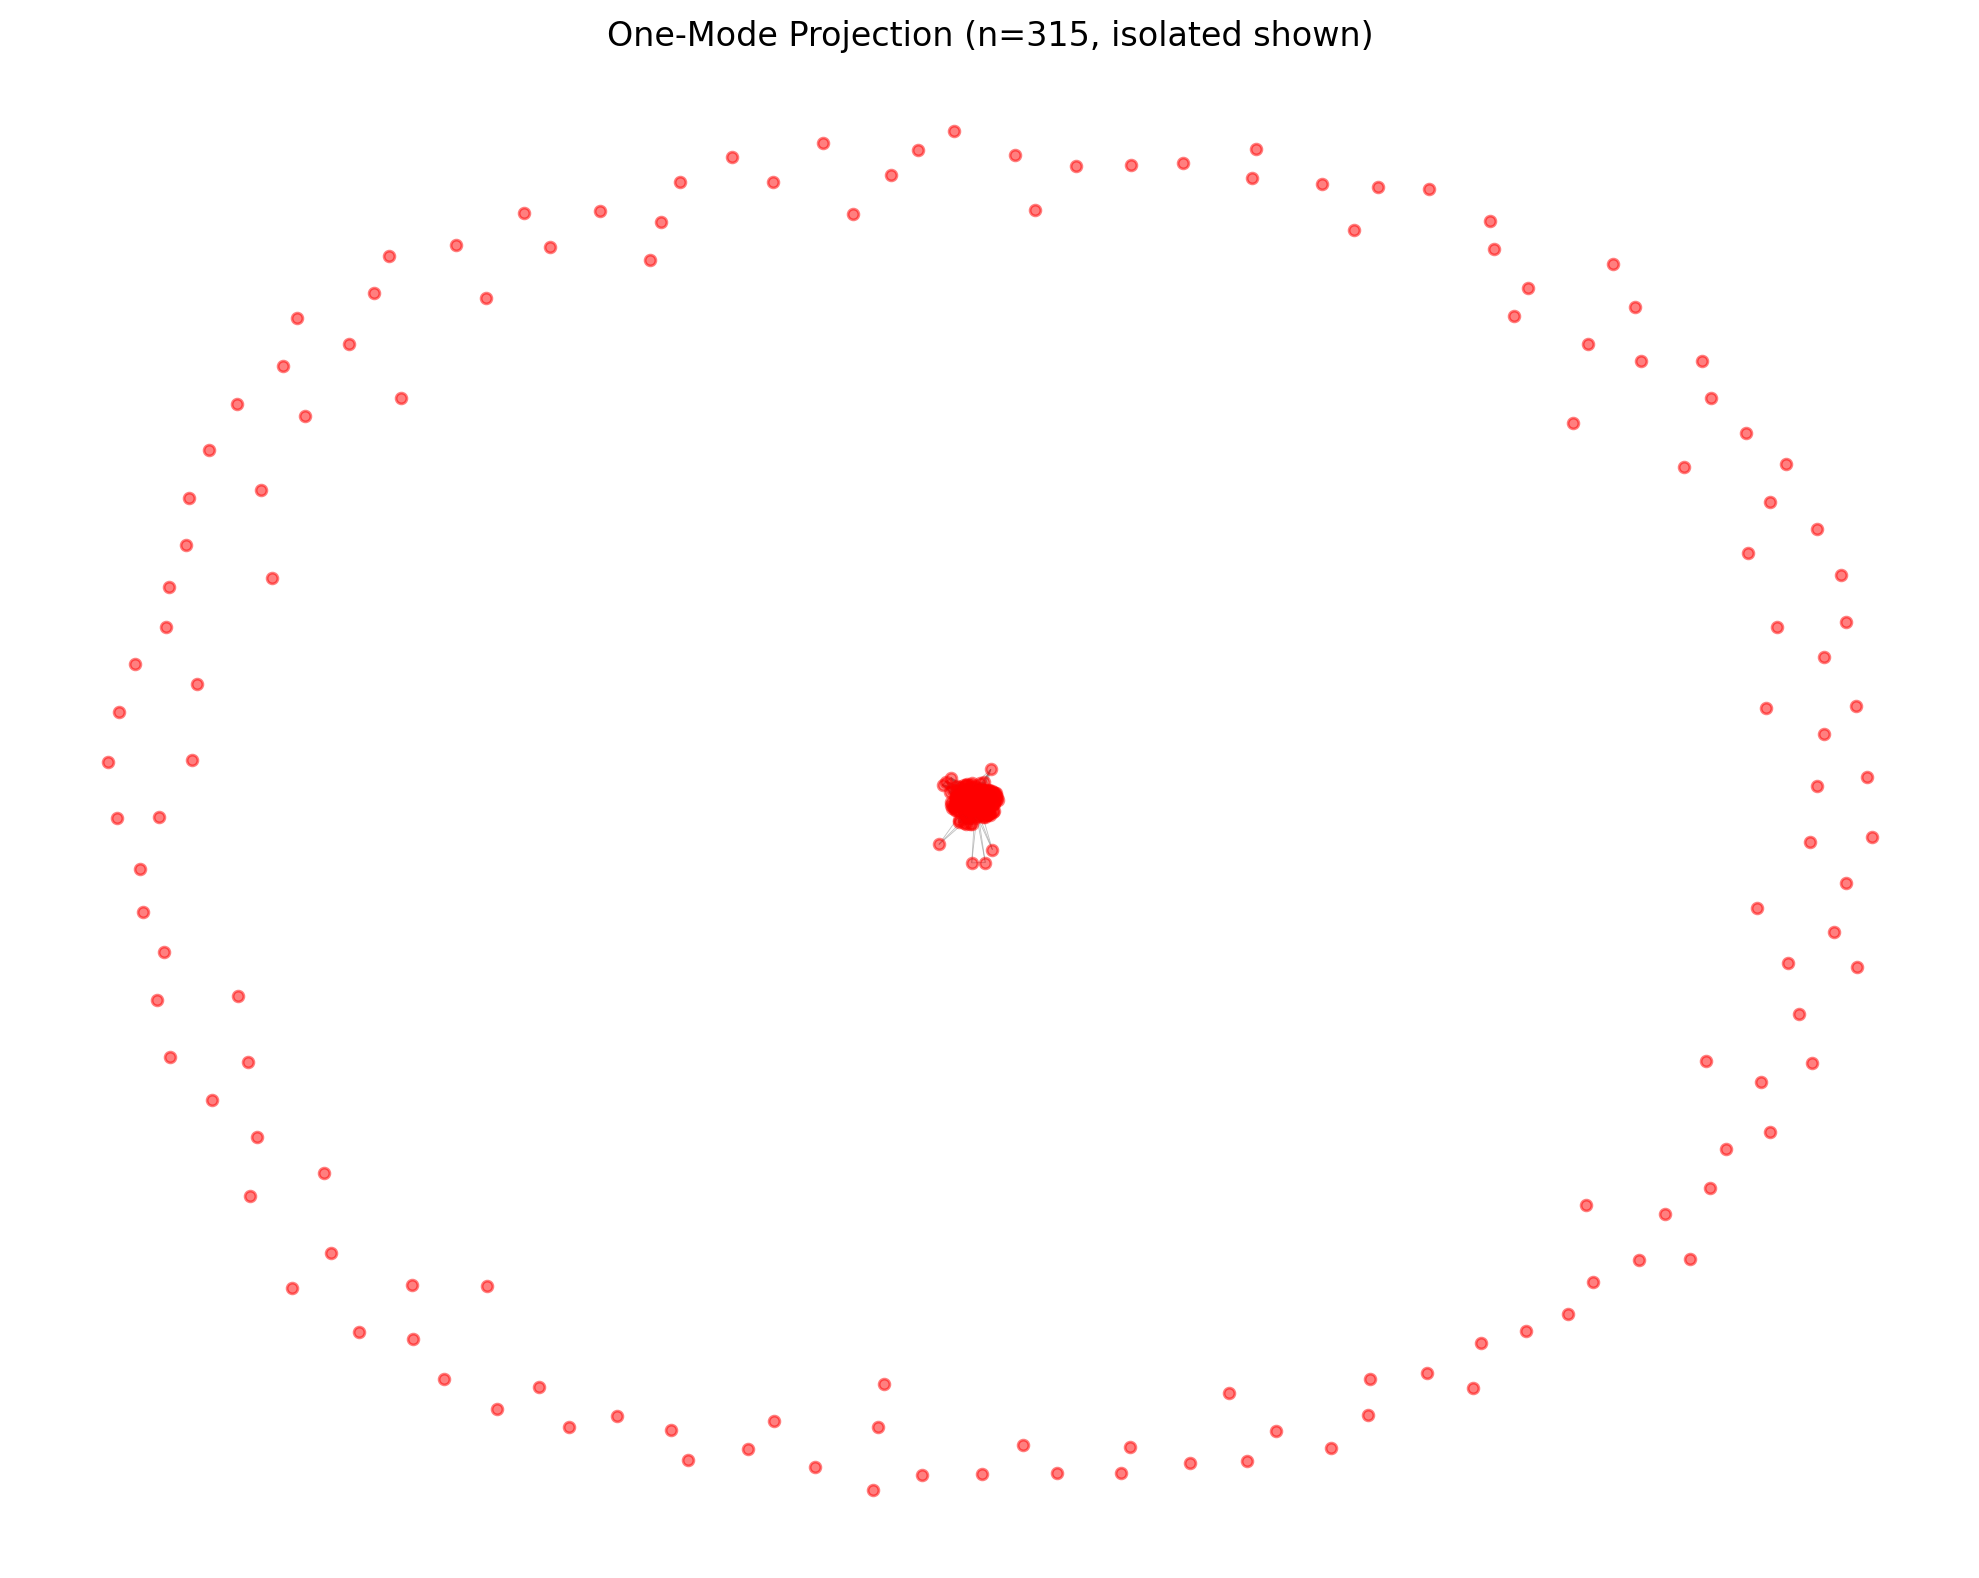
\includegraphics[width=\textwidth]{figs/one_mode_projection.png}
        \caption{Full projection (315 nodes)}
    \end{subfigure}
    \hfill
    \begin{subfigure}[b]{0.48\textwidth}
        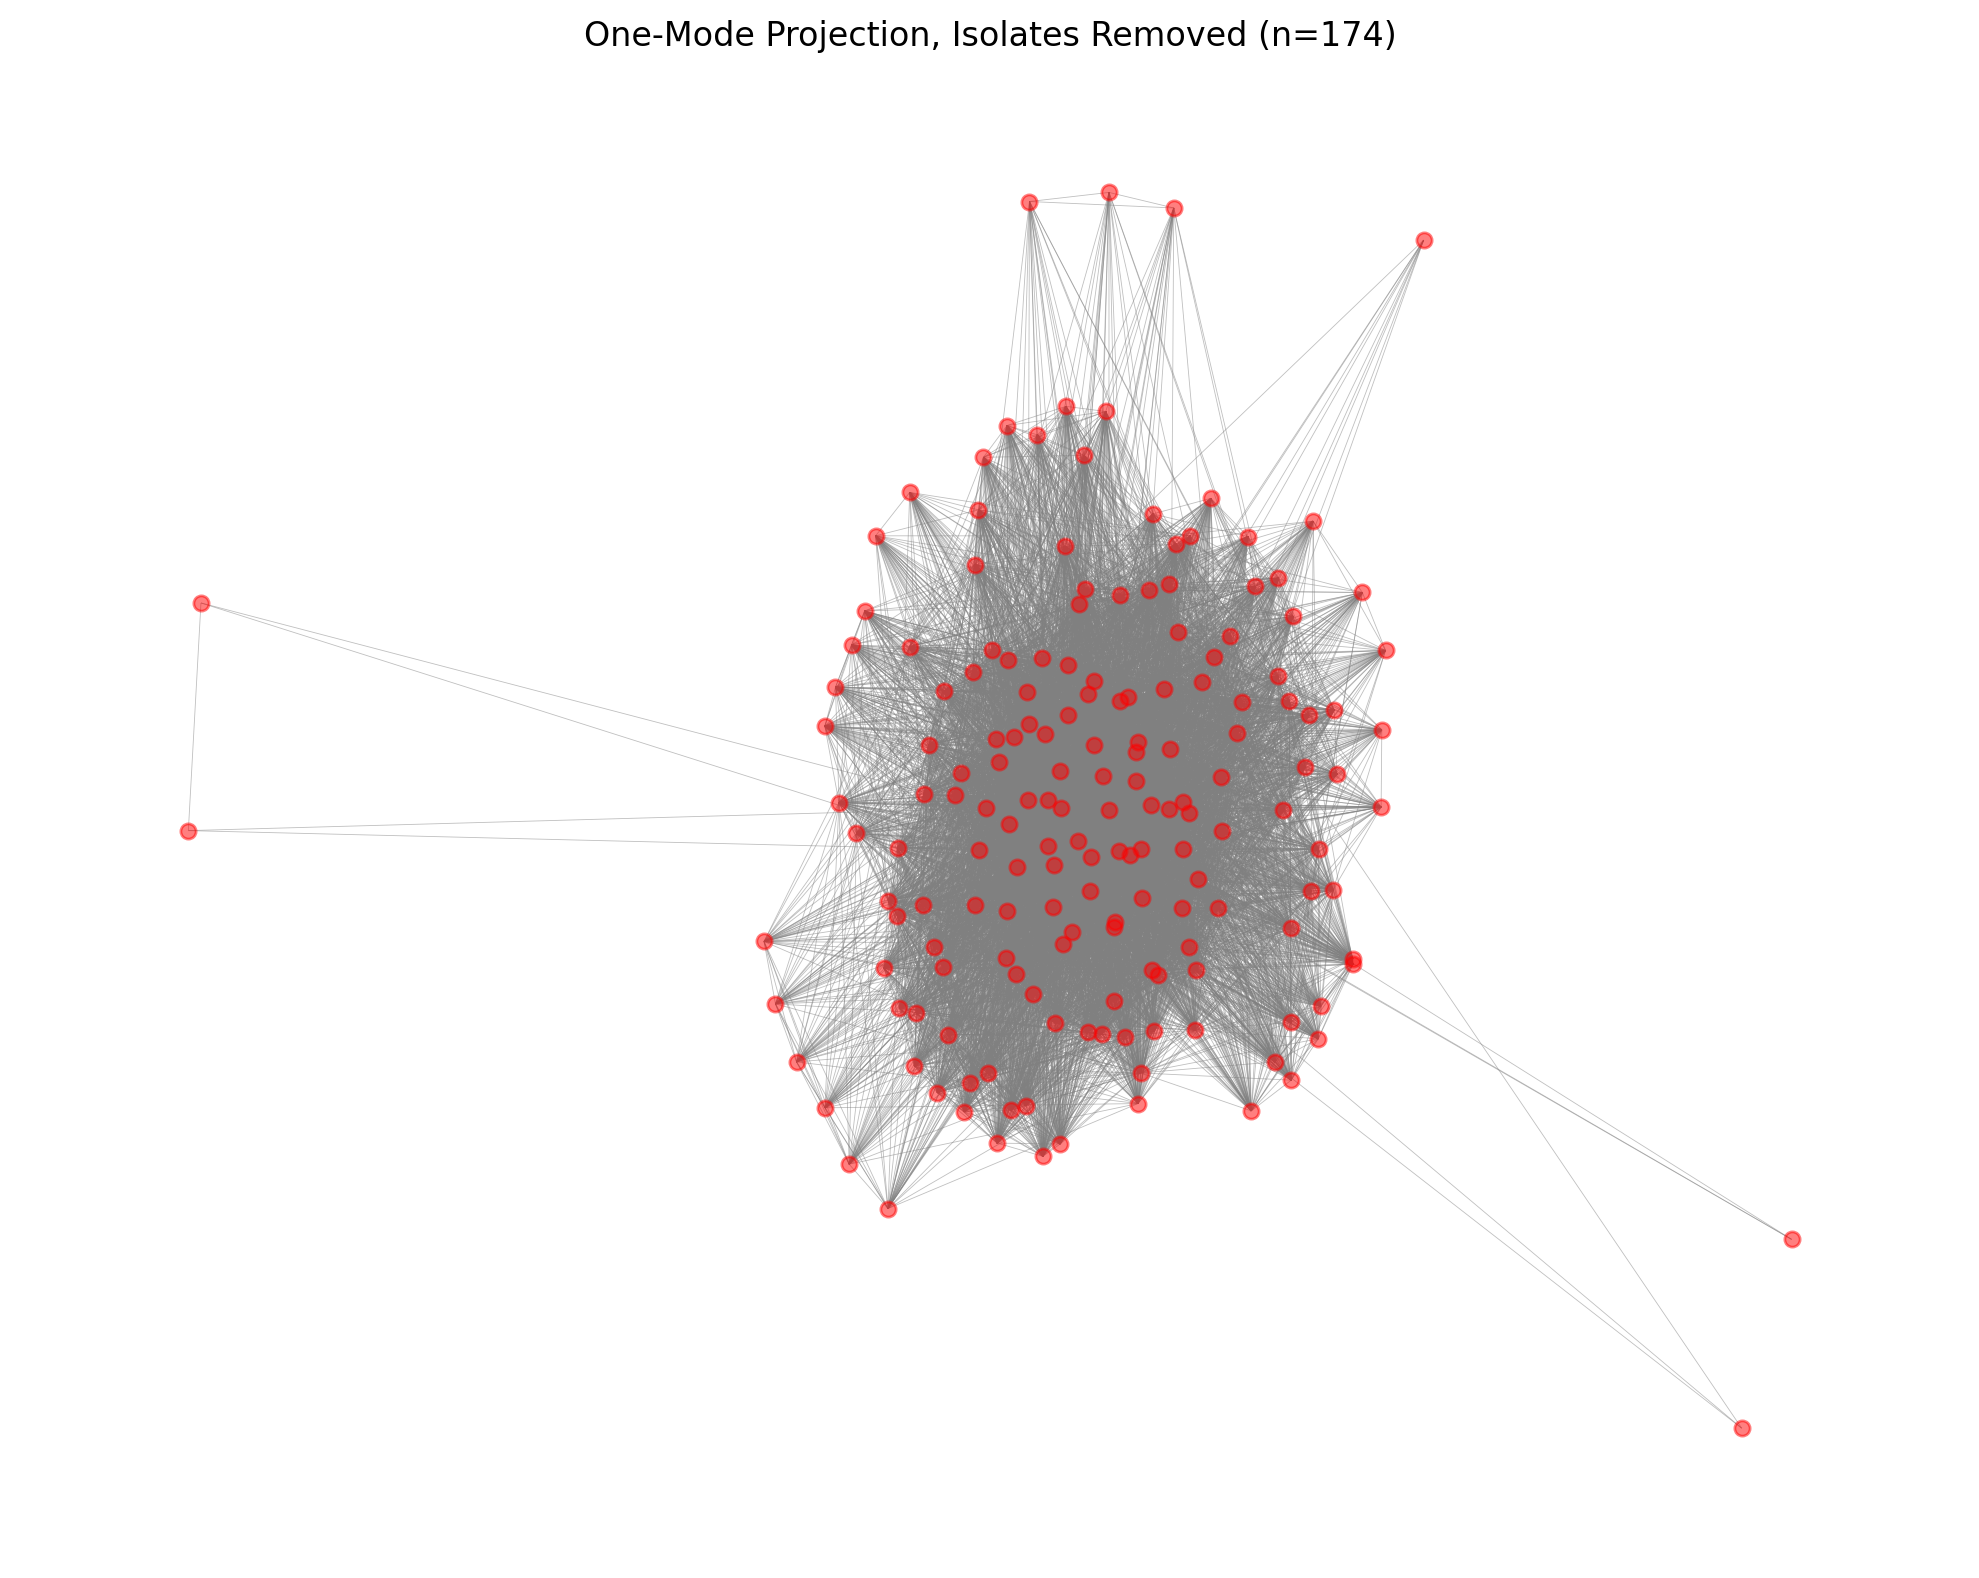
\includegraphics[width=\textwidth]{figs/one_mode_connected.png}
        \caption{Isolates removed (174 nodes)}
    \end{subfigure}
    \caption{One-mode projection of the knowledge graph onto a person-person network.}
    \label{fig:projection}
\end{figure}

The connected projection has a density of 0.578 and an average clustering coefficient of 0.853, indicating a tightly interconnected network where most users share many common contexts.

% =============================================================================
\section{Network Analysis}
% =============================================================================

All analysis from this point forward uses the connected projection graph (174 nodes, 8{,}704 edges).

\subsection{Centrality Measures}

I compute three centrality metrics to identify influential users:

\begin{itemize}
    \item \textbf{Degree centrality} -- the number of distinct users a node is connected to in the projected graph. High-degree nodes interact broadly across many threads and channels.
    \item \textbf{Eigenvector centrality} -- accounts not just for the number of connections but for the influence of those connections. A node scores high if it is connected to other high-scoring nodes.
    \item \textbf{PageRank} -- models importance as a random walk process, distributing influence through the network while accounting for connection structure.
\end{itemize}

\begin{table}[H]
\centering
\caption{Top 10 nodes by eigenvector centrality, with corresponding PageRank and degree. Role indicates TA or Student.}
\label{tab:centrality}
\begin{tabular}{clccc}
\toprule
Rank & Node & Eigenvec. Centrality & PageRank & Degree \\
\midrule
1  & 1 (TA)      & 0.1071 & 0.0094 & 169 \\
2  & 37 (Student) & 0.1067 & 0.0091 & 166 \\
3  & 87 (Student) & 0.1067 & 0.0093 & 166 \\
4  & 113 (Student) & 0.1067 & 0.0090 & 165 \\
5  & 222 (Student) & 0.1062 & 0.0094 & 166 \\
6  & 41 (TA)      & 0.1061 & 0.0091 & 165 \\
7  & 282 (Student) & 0.1060 & 0.0089 & 163 \\
8  & 310 (Student) & 0.1058 & 0.0096 & 164 \\
9  & 208 (Student) & 0.1056 & 0.0089 & 162 \\
10 & 158 (Student) & 0.1053 & 0.0088 & 160 \\
\bottomrule
\end{tabular}
\end{table}

The three metrics are highly correlated in this network. The top 10 nodes by each metric overlap substantially, which is consistent with the dense, core-periphery structure observed. Figures~\ref{fig:ec}--\ref{fig:degree} show each metric visualized as a heatmap over the network.

\begin{figure}[H]
    \centering
    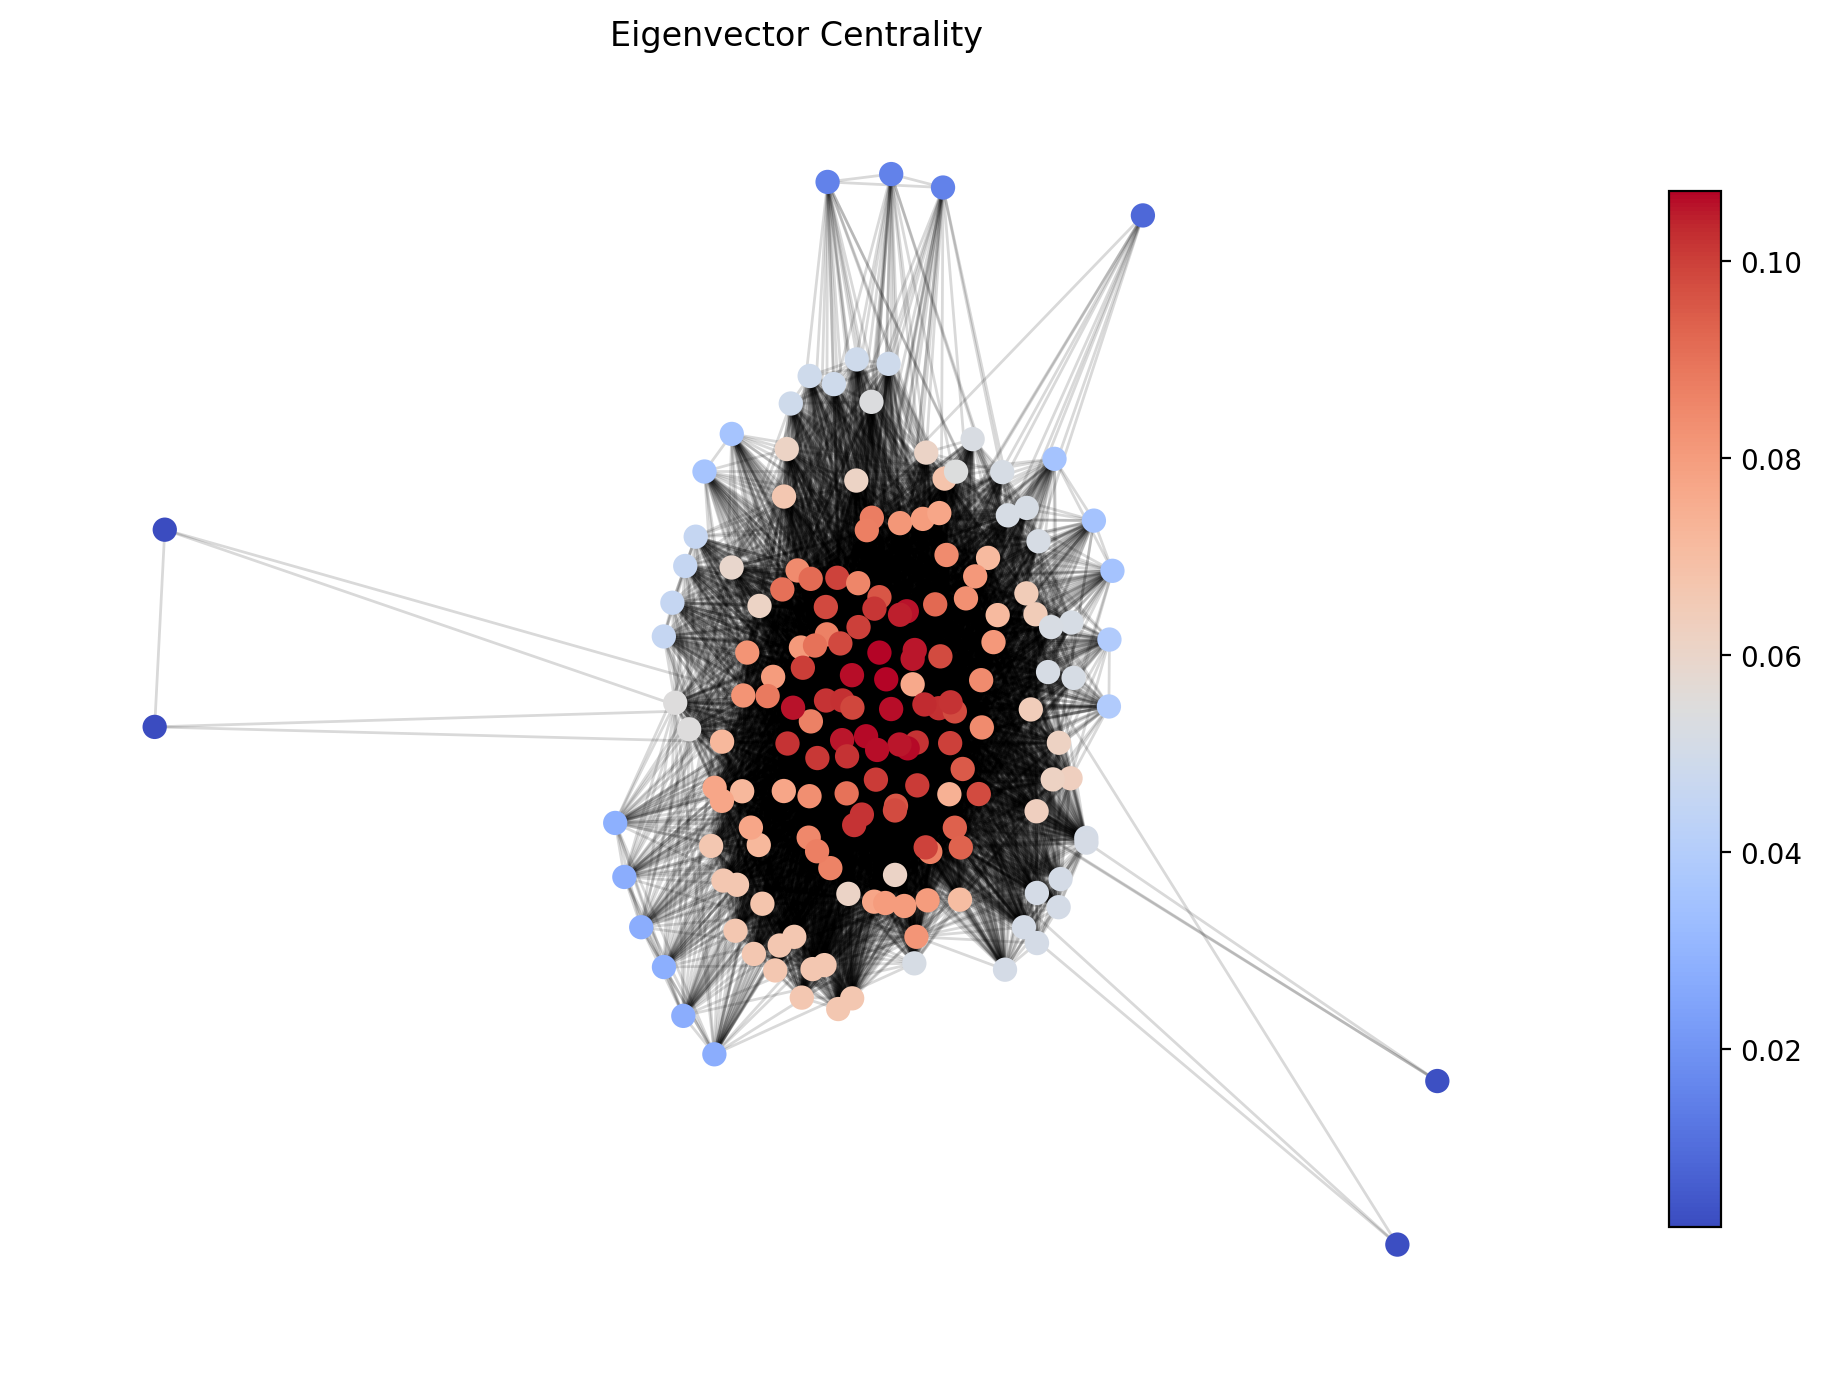
\includegraphics[width=0.75\textwidth]{figs/eigenvector_centrality.png}
    \caption{Nodes colored by eigenvector centrality. Warmer colors indicate higher centrality.}
    \label{fig:ec}
\end{figure}

\begin{figure}[H]
    \centering
    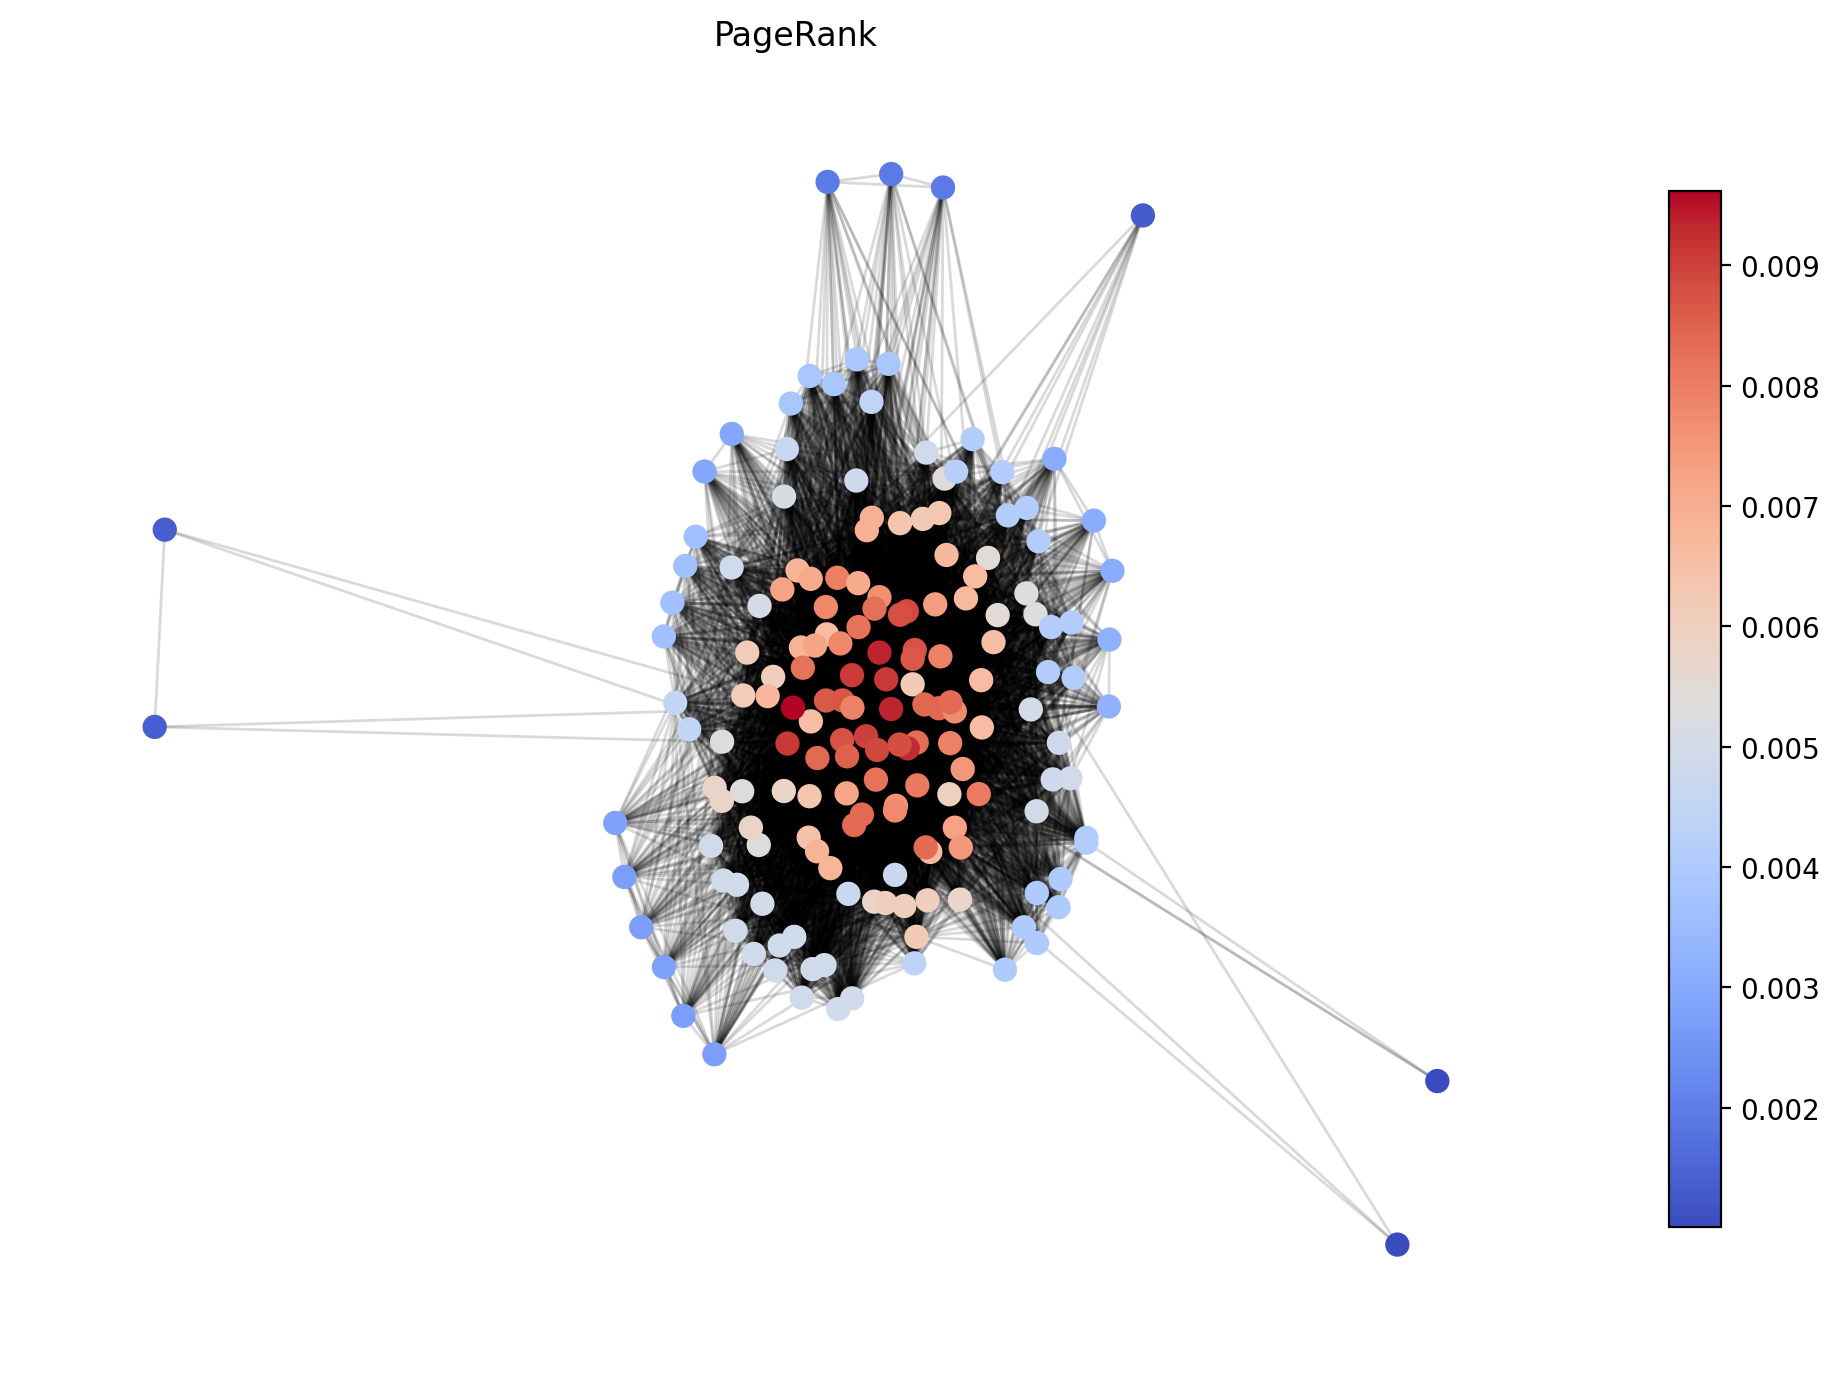
\includegraphics[width=0.75\textwidth]{figs/pagerank.png}
    \caption{Nodes colored by PageRank score.}
    \label{fig:pr}
\end{figure}

\begin{figure}[H]
    \centering
    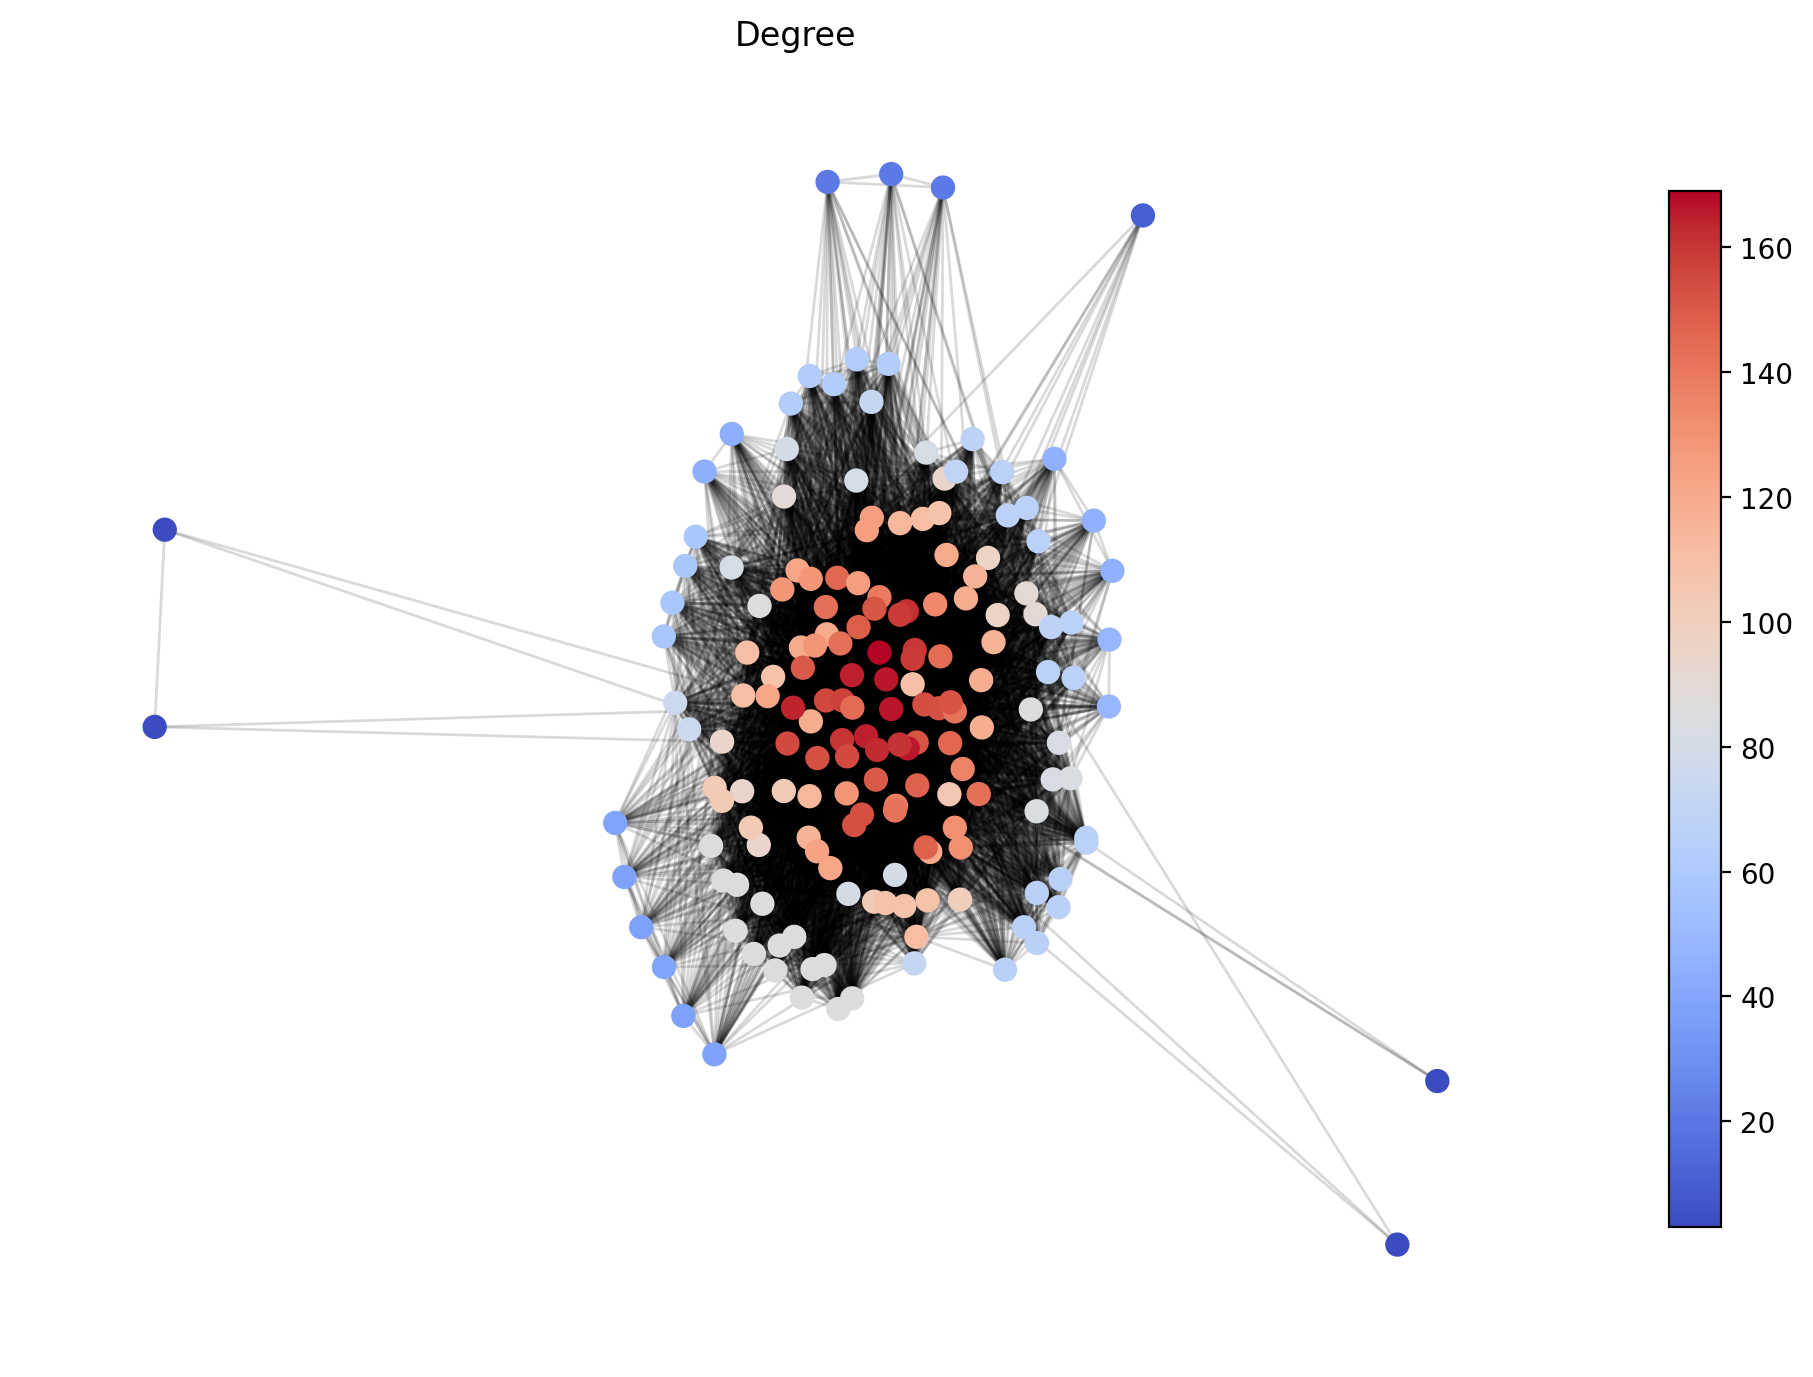
\includegraphics[width=0.75\textwidth]{figs/degree.png}
    \caption{Nodes colored by degree.}
    \label{fig:degree}
\end{figure}

\subsection{Identifying Key Nodes}

\textbf{TAs.} Of the 10 TAs in the connected network, 6 fall in the upper two quartiles across all three centrality metrics. The top two TAs (nodes 1 and 41) rank among the top 6 overall, making them natural candidates for seeding behavior adoption. TAs 83 and 75 are also well-positioned (ranks 16 and 20 by eigenvector centrality). The remaining 4 TAs (nodes 180, 23, 277, and three low-activity TAs at degree 21) are less central and would have limited reach as seeds.

\begin{table}[H]
\centering
\caption{All 10 TAs ranked by eigenvector centrality with quartile positions across metrics (4 = top quartile).}
\label{tab:tas}
\begin{tabular}{lccccc}
\toprule
Node & Eigenvec. Centrality & PageRank & Degree & EC Quartile \\
\midrule
1   & 0.1071 & 0.0094 & 169 & 4 \\
41  & 0.1061 & 0.0091 & 165 & 4 \\
83  & 0.1024 & 0.0087 & 157 & 4 \\
75  & 0.1021 & 0.0086 & 156 & 4 \\
180 & 0.0901 & 0.0072 & 129 & 3 \\
23  & 0.0808 & 0.0069 & 120 & 3 \\
277 & 0.0540 & 0.0044 &  73 & 2 \\
159 & 0.0151 & 0.0019 &  21 & 1 \\
168 & 0.0151 & 0.0019 &  21 & 1 \\
194 & 0.0151 & 0.0019 &  21 & 1 \\
\bottomrule
\end{tabular}
\end{table}

\textbf{Students.} The most influential students (nodes 37, 87, 113, 222, 282, 310, 208, 158, 304, 96) rival or exceed most TAs in centrality. These students are embedded deep in the network core and participate across many threads and channels. Their influence comes from broad participation rather than any institutional role, meaning they could serve as organic early adopters if targeted by TA-led interventions.

\subsection{Community Detection}

I applied four community detection algorithms to identify natural groupings:

\begin{enumerate}
    \item \textbf{Louvain clustering} (resolution = 0.95) -- identifies 3 communities with modularity $Q = 0.103$.
    \item \textbf{Newman hill-climbing} -- greedy modularity optimization, recursively applied to match the Louvain partition count.
    \item \textbf{Spectral modularity split} -- partitions using the leading eigenvector of the modularity matrix, recursively subdivided.
    \item \textbf{Normalized Laplacian graph cut} -- partitions using the Fiedler vector of the normalized Laplacian.
\end{enumerate}

\begin{figure}[H]
    \centering
    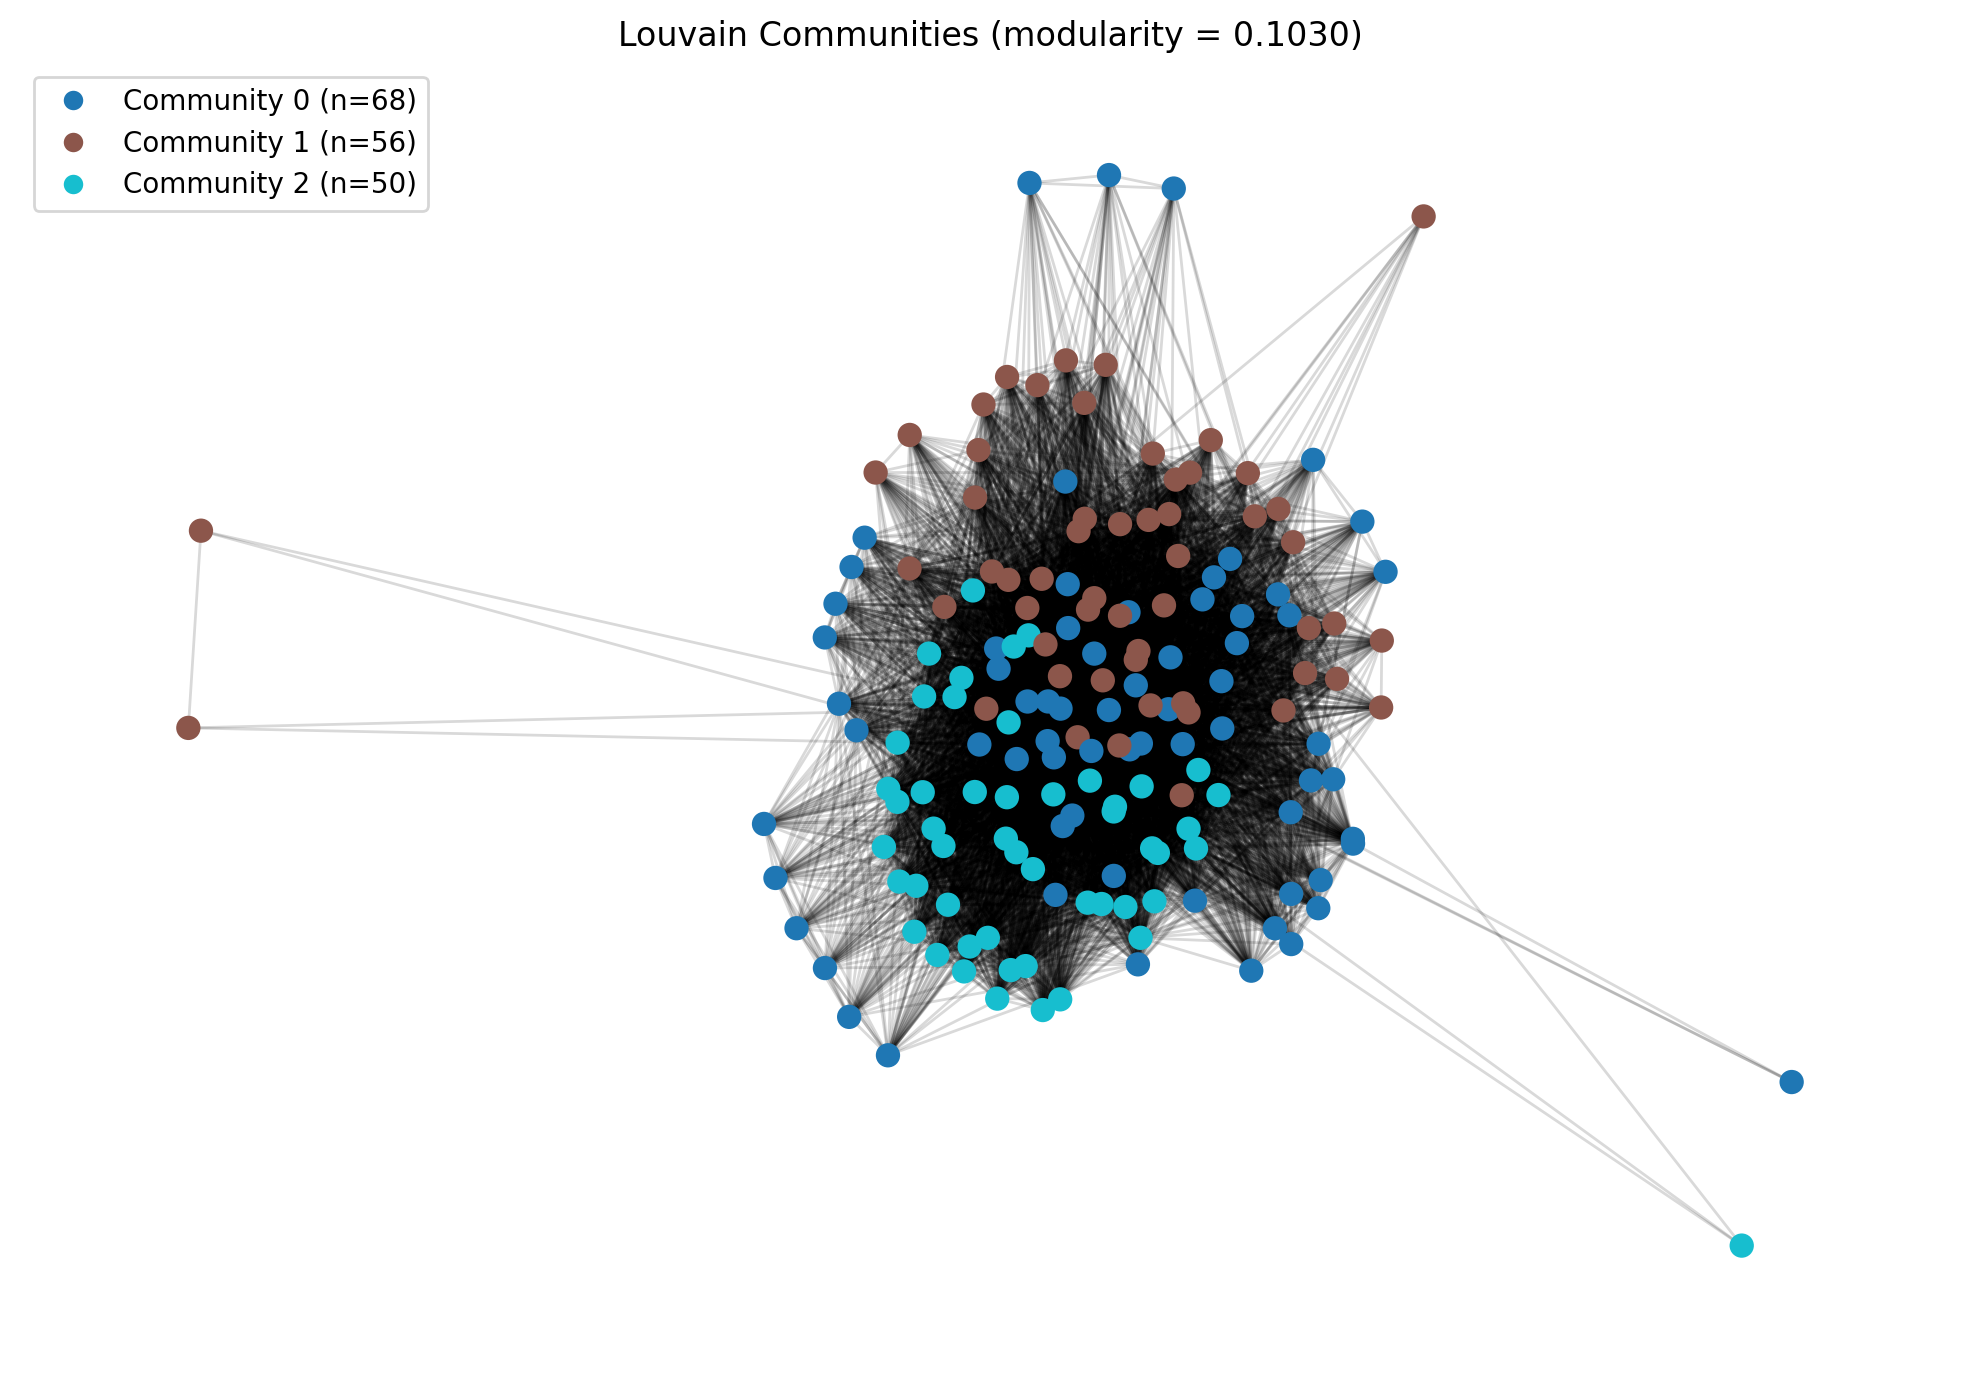
\includegraphics[width=0.75\textwidth]{figs/louvain_communities.png}
    \caption{Louvain community partition with 3 communities. Community sizes: 68, 56, and 50 nodes.}
    \label{fig:louvain}
\end{figure}

The low modularity ($Q \approx 0.1$) across all methods indicates that the network does not have strong community structure. This is consistent with the high density (0.578) and clustering coefficient (0.853): most nodes are connected to most other nodes, leaving little room for clear inter-community boundaries.

A k-core decomposition (Figure~\ref{fig:kcore}) confirms the core-periphery interpretation. The majority of nodes belong to a dense inner core, with a thin periphery of lower-degree nodes. This structure suggests that behavior spread is less about bridging separate communities and more about reaching the dense core, from which contagion can spread broadly.

\begin{figure}[H]
    \centering
    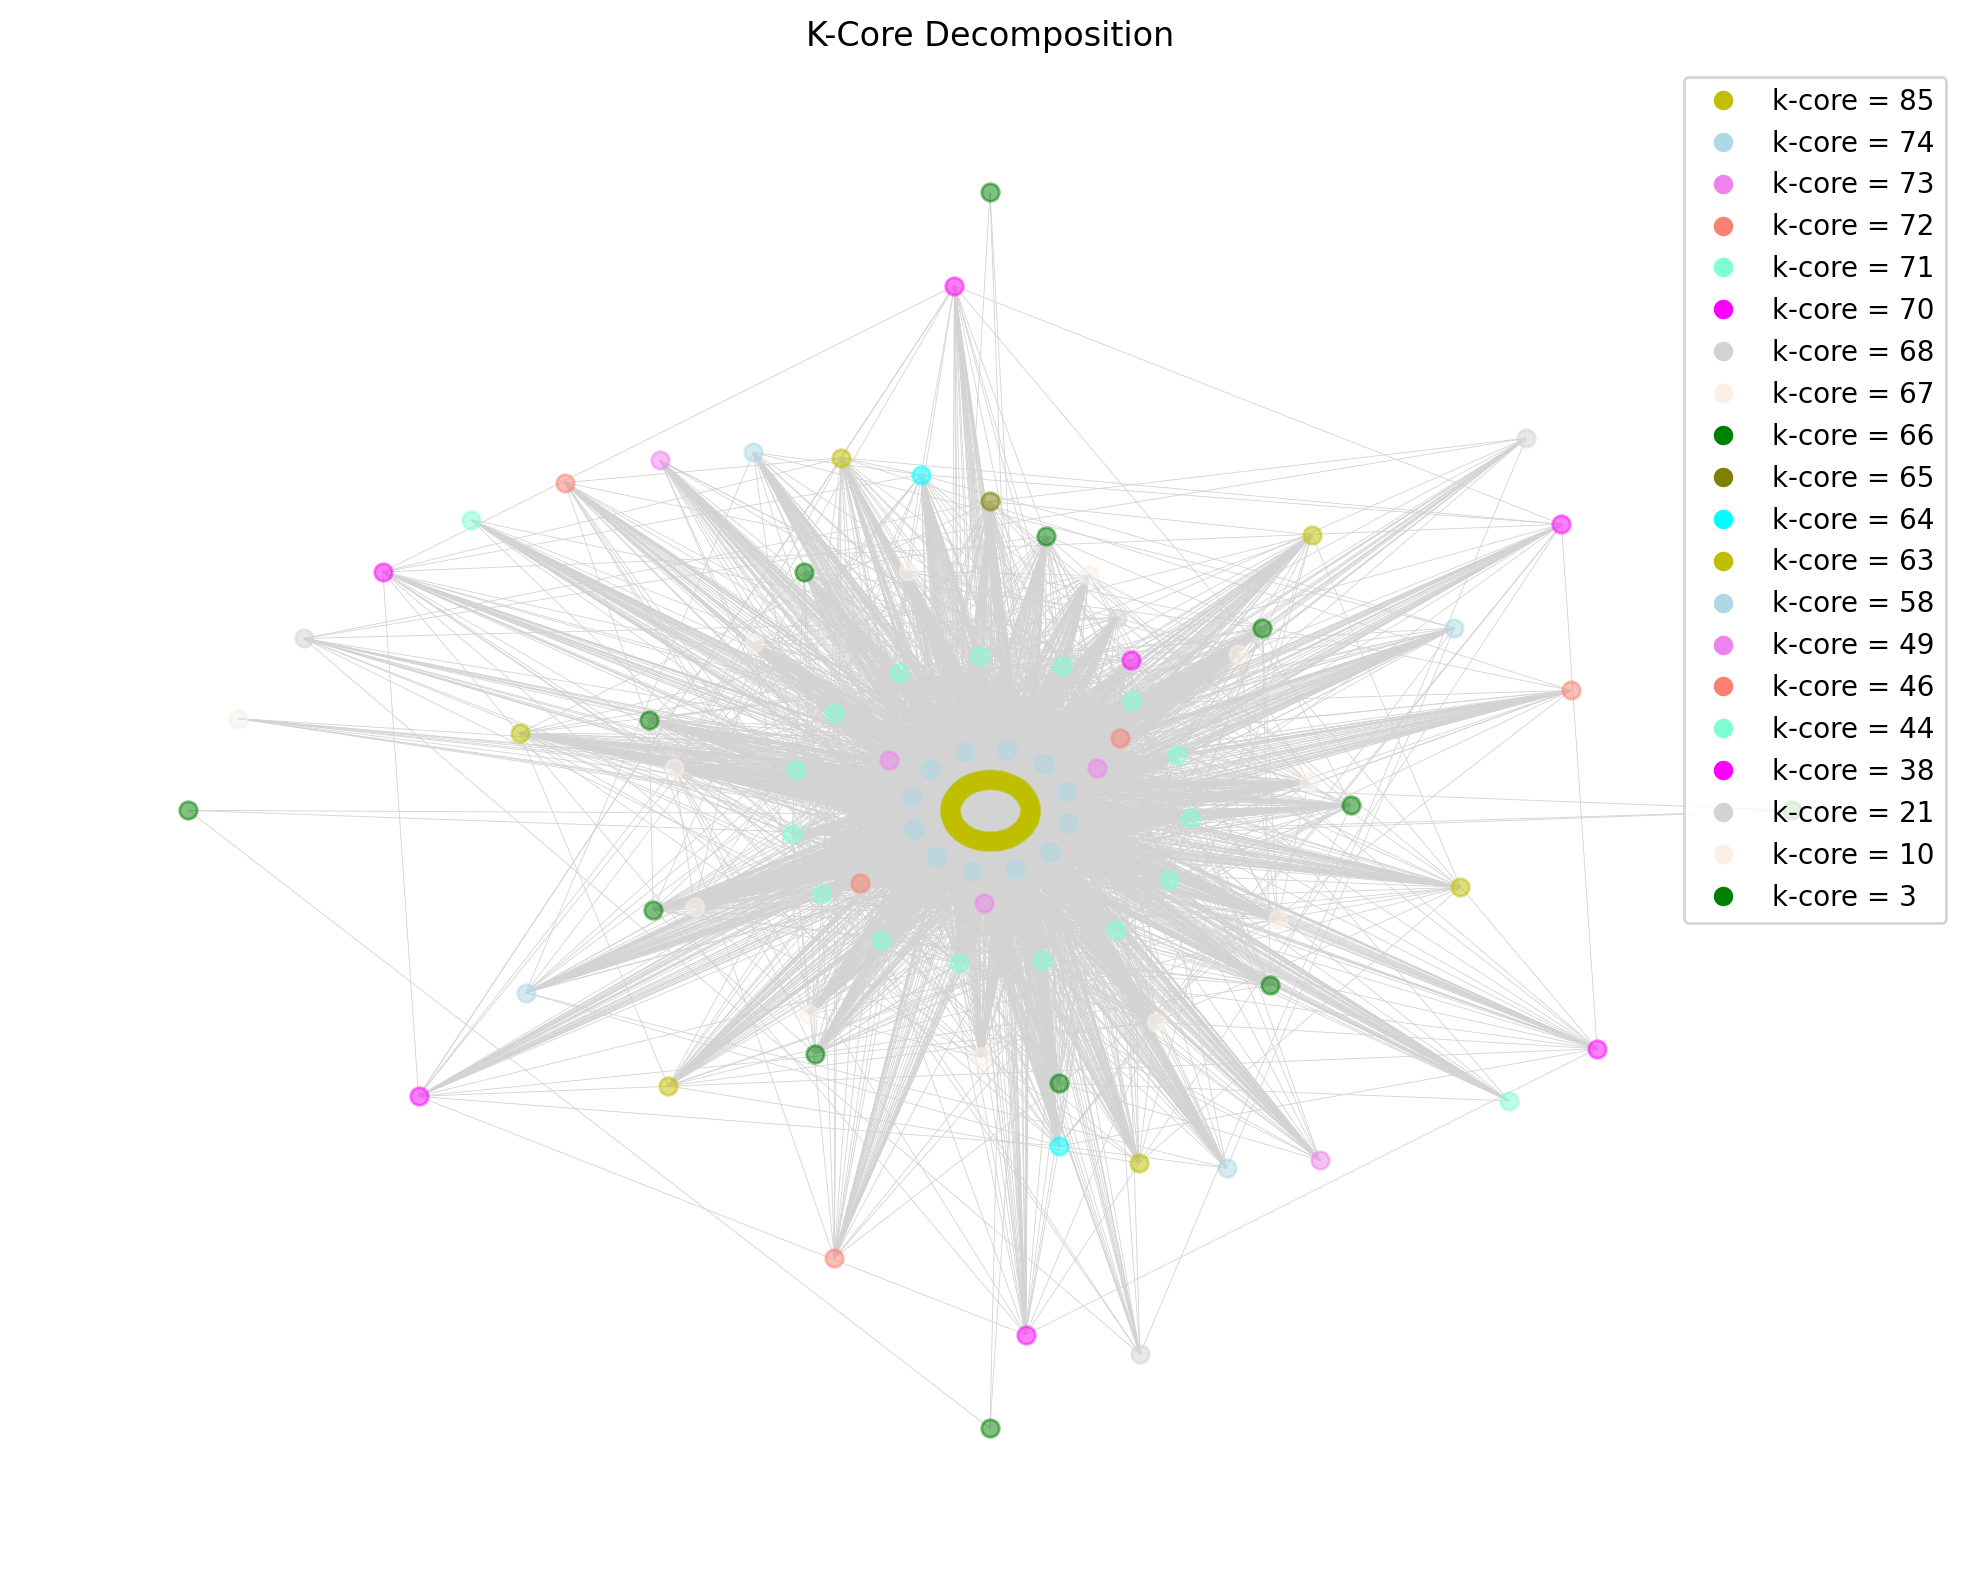
\includegraphics[width=0.75\textwidth]{figs/kcore.png}
    \caption{K-core decomposition. Most nodes belong to the high-k inner core, confirming core-periphery structure.}
    \label{fig:kcore}
\end{figure}

% =============================================================================
\section{Complex Contagion Simulation}
% =============================================================================

\subsection{Threshold Contagion Models}

I simulate behavior spread using synchronous threshold contagion. At each discrete time step, every non-adopted node evaluates whether its neighbors' adoption state meets a threshold criterion. Once adopted, a node remains adopted permanently. The simulation terminates when no new adoptions occur or after 20 steps.

I compare two threshold models:

\textbf{Absolute threshold model.} A node $v$ adopts at step $t+1$ if at least $k$ of its neighbors have adopted by step $t$:
\[
\bigl|\{u \in N(v) : u \text{ adopted at time } t\}\bigr| \geq k.
\]
I test $k \in \{2, 4, 5\}$. This models behaviors where exposure from a fixed number of distinct sources suffices---for example, hearing about a study technique from $k$ different peers.

\textbf{Fractional threshold model.} A node $v$ adopts at step $t+1$ if the fraction of adopted neighbors reaches threshold $\theta$:
\[
\frac{\bigl|\{u \in N(v) : u \text{ adopted at time } t\}\bigr|}{\deg(v)} \geq \theta.
\]
I test $\theta \in \{0.05, 0.10, 0.15, 0.20, 0.30, 0.40, 0.50\}$. This models behaviors requiring proportional social proof---a student adopts only when a significant share of their peers have done so.

The distinction matters greatly on dense networks. In the projected graph (average degree $\approx 100$), five adopted neighbors represent a meaningful absolute count but only ${\sim}5\%$ of a core node's neighborhood. As I show in Section~\ref{sec:sim_results}, this asymmetry causes the two models to produce dramatically different cascade outcomes.

\subsection{Early Adopter Selection Strategies}

I test five seeding strategies, selecting initial adopters based on the centrality analysis from Section~3:

\begin{enumerate}
    \item \textbf{Top $k$ TAs.} The highest-ranked TAs by eigenvector centrality, for $k \in \{1, 2, 3, 5\}$. The top 5 are nodes 1, 41, 83, 75, and 180 (degrees 169, 165, 157, 156, and 129).

    \item \textbf{Top 5 students.} The five highest-ranked students by eigenvector centrality: nodes 37, 87, 113, 222, and 282 (degrees 166, 166, 165, 166, and 163). Unlike the TA set, these nodes all have uniformly high degree.

    \item \textbf{Mixed (2\,TA + 3\,Student).} The top 2 TAs (nodes 1, 41) combined with the top 3 students (nodes 37, 87, 113), combining institutional authority with organic student influence.

    \item \textbf{Top $k$ overall.} The highest-ranked nodes by eigenvector centrality regardless of role, for $k \in \{5, 10, 20, 30\}$. At $k = 5$, this yields 1 TA and 4 students.

    \item \textbf{Random.} Five randomly selected nodes, providing a non-targeted baseline.
\end{enumerate}

These strategies enable comparison across three dimensions: role (TAs vs.\ students vs.\ mixed), targeting (centrality-based vs.\ random), and scale (how many seeds are required for cascade).

\subsection{Simulation Results}
\label{sec:sim_results}

\textbf{Absolute threshold results.}
Under the absolute threshold model, a sharp phase transition emerges at the boundary between the seed count and the threshold $k$ (Table~\ref{tab:abs_phase}). When the number of seeds is less than $k$, no node can meet the adoption criterion at step~1, and no cascade occurs. With 5 seeds, near-complete adoption occurs within 2 steps regardless of strategy.

\begin{table}[H]
\centering
\caption{Phase transition in the absolute threshold model. With fewer seeds than the threshold $k$, no cascade occurs. Seeds are the top TAs by eigenvector centrality.}
\label{tab:abs_phase}
\begin{tabular}{lccc}
\toprule
Seeds & $k = 2$ & $k = 4$ & $k = 5$ \\
\midrule
1 (Top 1 TA) & --- & 0.6\% & 0.6\% \\
2 (Top 2 TAs) & 100\% & 1.1\% & 1.1\% \\
3 (Top 3 TAs) & --- & 1.7\% & 1.7\% \\
5 (Top 5 TAs) & 100\% & 97.7\% & 97.7\% \\
\bottomrule
\end{tabular}
\end{table}

With $k \geq 4$ and only 1--3 seeds, no cascade is possible: each node's maximum number of adopted neighbors equals the seed count, which falls below the threshold. This is a structural guarantee, not a consequence of poor seed placement. The four nodes that never adopt under $k \geq 4$ (nodes 139, 167, 188, and 250) have degree~3 and share no edges with any seed node. With only 3 neighbors, they cannot reach a threshold of 4 regardless of how the cascade unfolds elsewhere.

While all 5-seed strategies converge to the same final adoption, they differ in step-1 speed. Table~\ref{tab:abs_strategy} compares strategies under $k = 5$, the most discriminating threshold.

\begin{table}[H]
\centering
\caption{Strategy comparison under absolute threshold $k = 5$. All strategies reach 97.7\% by step~2; step-1 adoption reveals speed differences.}
\label{tab:abs_strategy}
\begin{tabular}{lc}
\toprule
Strategy & Step 1 Adopted (of 174) \\
\midrule
Top 5 Students      & 163 \\
Mixed 2\,TA + 3\,S  & 163 \\
Top 5 TAs           & 125 \\
Random (5)          &  41 \\
\bottomrule
\end{tabular}
\end{table}

Top students and the mixed strategy both achieve 163 adoptions at step~1, outperforming the TA-only strategy by 30\%. This gap arises from the TA set's uneven degree distribution: the 5th-ranked TA (node 180, degree 129) reaches only 74\% of the network, while the 5th-ranked student (node 282, degree 163) reaches 94\%. Consequently, 158 non-seed nodes share edges with all 5 top students, compared to only 120 for the top 5 TAs. Random seeding is slowest (41 at step~1) but still converges by step~2 due to the dense core.

\textbf{Fractional threshold results.}
The fractional threshold model yields dramatically different results. Table~\ref{tab:frac_sweep} shows that with 5 seeds, a critical transition occurs between $\theta = 0.10$ and $\theta = 0.15$: below this boundary, full cascade occurs; above it, adoption stalls near the seed count.

\begin{table}[H]
\centering
\caption{Fractional threshold results with 5 seeds. Full cascade occurs only at $\theta \leq 0.10$. Steps indicates the number of time steps to full adoption; ``---'' indicates that the cascade stalls.}
\label{tab:frac_sweep}
\begin{tabular}{lcccc}
\toprule
$\theta$ & Top 5 TAs & Top 5 Students & Mixed 2\,TA+3\,S & Steps \\
\midrule
0.05 & 100\% & 100\% & 100\% & 3 \\
0.10 & 100\% & 100\% & 100\% & 4 \\
\midrule
0.15 & 4.6\% & 4.6\% & 4.0\% & --- \\
0.20 & 4.6\% & 4.6\% & 4.0\% & --- \\
0.30 & 2.9\% & 4.6\% & 3.4\% & --- \\
0.50 & 2.9\% & 3.4\% & 2.9\% & --- \\
\bottomrule
\end{tabular}
\end{table}

The failure at $\theta \geq 0.15$ follows directly from the network's density: with 5 seeds and average degree ${\approx}100$, a core node sees at most $5/100 = 5\%$ of its neighbors adopted at step~1, far below the 15\% threshold. Only a handful of extreme periphery nodes (degree $\leq 10$) can cross the threshold, and their adoption does not propagate further into the dense core.

At $\theta = 0.10$, a qualitatively different cascade emerges (Figure~\ref{fig:frac_transition}). Rather than the near-instantaneous step-function behavior of the absolute model, adoption builds gradually: with top 5 TAs, the cascade proceeds as $5 \to 15 \to 24 \to 78 \to 174$. Low-degree periphery nodes adopt first (steps 1--2), then once enough intermediate nodes have converted, core nodes are pushed past the 10\% threshold, triggering an explosive wave at step~3. This S-shaped buildup is characteristic of complex contagion.

\begin{figure}[H]
    \centering
    \begin{subfigure}[b]{0.32\textwidth}
        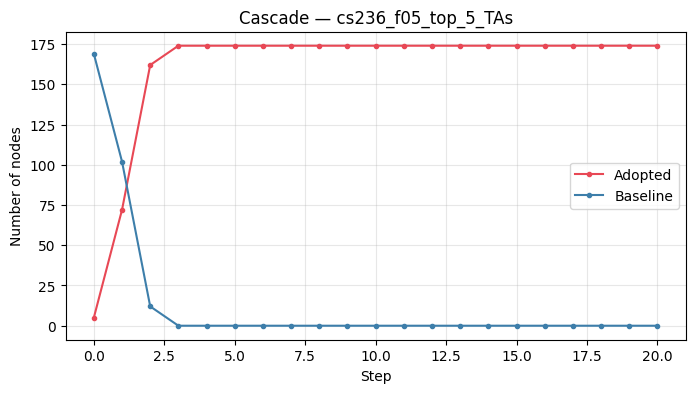
\includegraphics[width=\textwidth]{../data/cs236/cs236_f05_top_5_TAs/cascade.png}
        \caption{$\theta = 0.05$ (3 steps)}
    \end{subfigure}
    \hfill
    \begin{subfigure}[b]{0.32\textwidth}
        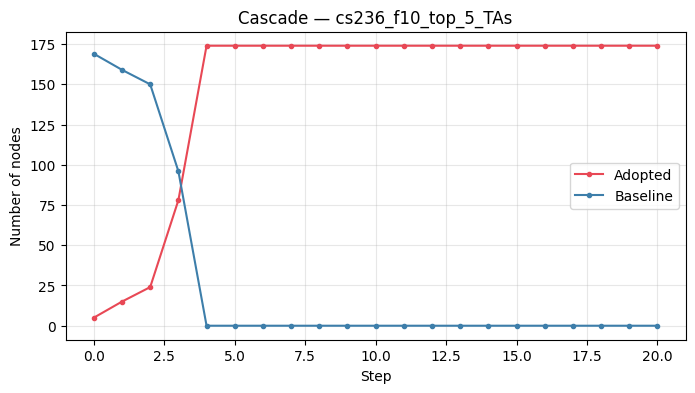
\includegraphics[width=\textwidth]{../data/cs236/cs236_f10_top_5_TAs/cascade.png}
        \caption{$\theta = 0.10$ (4 steps)}
    \end{subfigure}
    \hfill
    \begin{subfigure}[b]{0.32\textwidth}
        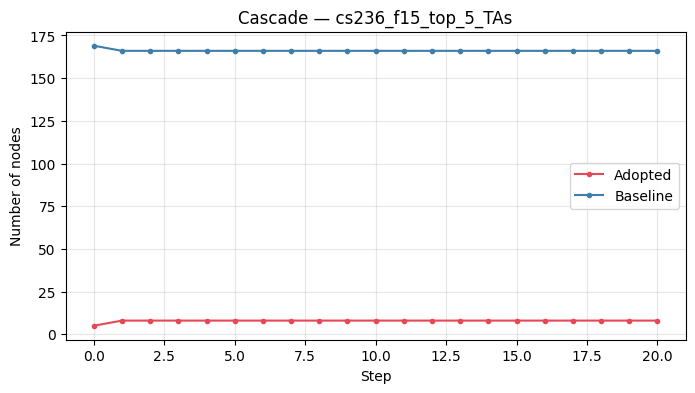
\includegraphics[width=\textwidth]{../data/cs236/cs236_f15_top_5_TAs/cascade.png}
        \caption{$\theta = 0.15$ (stalls at 4.6\%)}
    \end{subfigure}
    \caption{Cascade dynamics under fractional thresholds with top 5 TAs as seeds, showing the critical transition between $\theta = 0.10$ (full cascade) and $\theta = 0.15$ (failure).}
    \label{fig:frac_transition}
\end{figure}

\textbf{Seed count scaling.}
For fractional thresholds above the critical value, increasing the number of seeds can restore cascade. Table~\ref{tab:seed_scaling} shows results for $\theta = 0.20$ and $\theta = 0.30$ with 10, 20, and 30 seeds selected by eigenvector centrality regardless of role.

\begin{table}[H]
\centering
\caption{Seed count scaling under fractional thresholds. Seeds are the top nodes by eigenvector centrality. With 5 seeds, both thresholds fail to cascade (Table~\ref{tab:frac_sweep}).}
\label{tab:seed_scaling}
\begin{tabular}{lccc}
\toprule
$\theta$ & 10 seeds & 20 seeds & 30 seeds \\
\midrule
0.20 & 100\% (7 steps) & 100\% (3 steps) & 100\% (2 steps) \\
0.30 & 7.5\% (stalls) & 100\% (4 steps) & 100\% (3 steps) \\
\bottomrule
\end{tabular}
\end{table}

At $\theta = 0.20$, 10 seeds is the minimum tested count for full cascade, but the process is slow: adoption builds over 7 steps ($10 \to 24 \to 28 \to 31 \to 36 \to 59 \to 159 \to 174$), with a long smoldering phase before a tipping point at steps~5--6 where adoption suddenly accelerates (Figure~\ref{fig:seed_scaling}). Doubling to 20 seeds reduces convergence to 3 steps; 30 seeds produces near-instant adoption in 2 steps, resembling the absolute model.

At $\theta = 0.30$, 10 seeds is insufficient (stalls at 7.5\%), but 20 seeds achieves full cascade in 4 steps. Higher thresholds require proportionally more seeds: roughly 6\% of the network at $\theta = 0.20$ and 12\% at $\theta = 0.30$.

\begin{figure}[H]
    \centering
    \begin{subfigure}[b]{0.32\textwidth}
        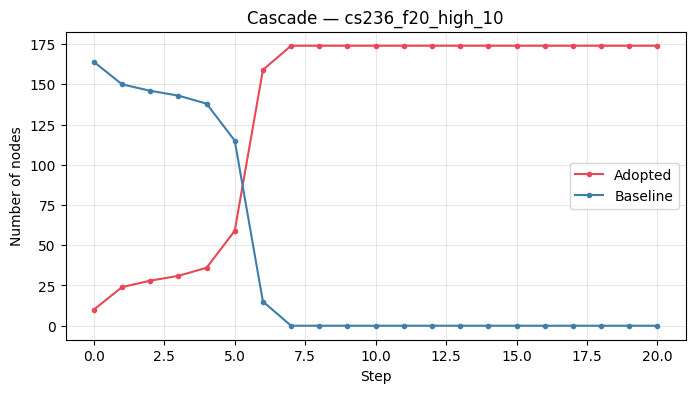
\includegraphics[width=\textwidth]{../data/cs236/cs236_f20_high_10/cascade.png}
        \caption{10 seeds (7 steps)}
    \end{subfigure}
    \hfill
    \begin{subfigure}[b]{0.32\textwidth}
        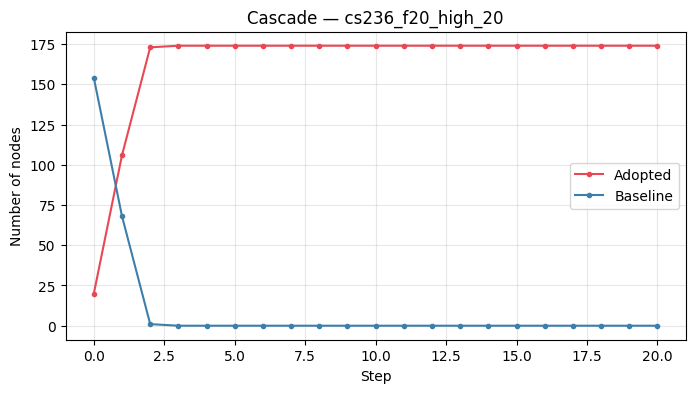
\includegraphics[width=\textwidth]{../data/cs236/cs236_f20_high_20/cascade.png}
        \caption{20 seeds (3 steps)}
    \end{subfigure}
    \hfill
    \begin{subfigure}[b]{0.32\textwidth}
        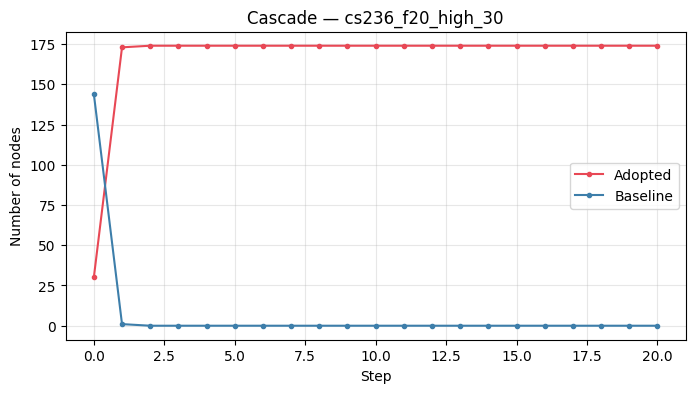
\includegraphics[width=\textwidth]{../data/cs236/cs236_f20_high_30/cascade.png}
        \caption{30 seeds (2 steps)}
    \end{subfigure}
    \caption{Effect of seed count on cascade dynamics at $\theta = 0.20$. With 10 seeds, adoption smolders for 5 steps before a tipping point. With 30 seeds, convergence is near-instant.}
    \label{fig:seed_scaling}
\end{figure}

% =============================================================================
\section{Optimizing Behavior Adoption}
% =============================================================================

\subsection{Intervention Strategies}

The simulation results motivate three intervention strategies, each suited to different assumptions about how behavior adoption works:

\textbf{Strategy A: Targeted seeding under absolute contagion.} If adoption follows an absolute threshold (a student needs to hear from $k$ distinct adopters), a small set of 5 well-chosen seeds achieves near-complete adoption. The key intervention is selecting seeds that collectively maximize network coverage. My results show that the top 5 students or a mixed TA--student set outperforms TA-only seeding, because the top students have more uniformly high degree. TAs 1 and 41 should still be included for their institutional authority, combined with the most active students.

\textbf{Strategy B: Threshold reduction under fractional contagion.} If adoption requires proportional social proof, the most cost-effective intervention is reducing the effective threshold rather than adding more seeds. With 5 seeds, cascade succeeds at $\theta \leq 0.10$ but fails at $\theta \geq 0.15$. Pedagogical approaches that lower the barrier---such as making target behaviors visible, providing starter templates, or integrating them into graded course structure---can shift $\theta$ from the ``hard'' regime into the ``easy'' regime without requiring additional seeds.

\textbf{Strategy C: Seed scaling under high fractional thresholds.} When the threshold cannot be lowered (e.g., behaviors that inherently require strong social proof), more seeds are needed. At $\theta = 0.20$, 10 seeds (6\% of the network) suffice; at $\theta = 0.30$, 20 seeds (12\%) are required. These seeds should be selected by eigenvector centrality regardless of role, as the top-overall strategy benefits from uniformly high connectivity.

\subsection{Justification of Methods}

The choice of centrality measures is motivated by the network's structure. Because the projected network is dense and exhibits core-periphery organization rather than distinct communities, eigenvector centrality is particularly appropriate: it captures not just how many connections a node has, but whether those connections themselves are well-connected. In this network, nodes with high eigenvector centrality sit at the heart of the core and can influence the largest fraction of the network through short paths.

PageRank provides a complementary view by modeling influence as a diffusion process, which aligns with how information and behaviors spread through a social network. The close agreement between degree, eigenvector centrality, and PageRank in this network reinforces that the central nodes are robust influence points regardless of the specific metric used.

Community detection, while yielding low modularity, still provides value: even weak community boundaries suggest subgroups that may require separate seed nodes to ensure contagion reaches all parts of the network. The Louvain partition, despite its modest modularity, identifies three groups that can guide the placement of early adopters to ensure no subgroup is left unseeded.

\subsection{Results and Analysis}

The choice of contagion model fundamentally determines the intervention strategy. Under the absolute threshold model ($k \leq 5$), behavior adoption is easy to initiate: 5 central seeds produce 97.7--100\% adoption in 2 steps regardless of the specific seeding strategy. The network's high density ensures that once a critical mass of seeds is placed in the core, the cascade propagates through the dense interconnections. In this regime, the intervention problem reduces to ensuring that the seed count exceeds $k$ and that seeds are not all concentrated among low-degree nodes.

Under the fractional threshold model, the same density that enables absolute cascades becomes an obstacle. Each seed's influence is diluted across many connections, making it difficult for any node to reach the proportional threshold. The critical boundary at $\theta \approx 0.10\text{--}0.15$ with 5 seeds corresponds directly to the ratio $k_{\text{seeds}} / \bar{d}$: five seeds divided by the average degree of ${\approx}100$ yields an effective contribution of ${\sim}5\%$, sufficient for $\theta = 0.05$ but not $\theta = 0.15$.

Table~\ref{tab:tradeoff} summarizes the minimum tested seed count that achieves full cascade under each model configuration.

\begin{table}[H]
\centering
\caption{Minimum tested seed count achieving full cascade under each model. Seeds selected by eigenvector centrality.}
\label{tab:tradeoff}
\begin{tabular}{lcc}
\toprule
Model \& Threshold & Min.\ Seeds for Cascade & \% of Network \\
\midrule
Absolute, $k = 2$ & 2 & 1.1\% \\
Absolute, $k = 4$ & 5 & 2.9\% \\
Absolute, $k = 5$ & 5 & 2.9\% \\
Fractional, $\theta = 0.05$ & 5 & 2.9\% \\
Fractional, $\theta = 0.10$ & 5 & 2.9\% \\
Fractional, $\theta = 0.20$ & 10 & 5.7\% \\
Fractional, $\theta = 0.30$ & 20 & 11.5\% \\
\bottomrule
\end{tabular}
\end{table}

The practical implication is clear: if course designers can engineer conditions where adoption follows an absolute model (e.g., through structured peer exposure or explicit endorsements), a small number of targeted interventions suffice. If adoption is inherently proportional, the required investment scales with the threshold---either through recruiting more early adopters or through structural changes that lower $\theta$.

Among seeding strategies, the mixed TA--student approach emerges as the most robust choice. It matches or exceeds TA-only seeding in every configuration tested, leveraging the institutional credibility of TAs for legitimacy and the broad connectivity of top students for reach. The TA-only strategy's weakness stems from the uneven degree distribution among TAs: while TAs 1 and 41 are among the most central nodes in the network, the remaining TAs drop off sharply (node 180 has degree 129 vs.\ the top students' uniform ${\sim}165$).

% =============================================================================
\section{Recommendations}
% =============================================================================

Based on the network analysis and contagion simulations, I offer the following strategies for maximizing behavior adoption:

\begin{enumerate}
    \item \textbf{Use mixed TA--student seeding.} The mixed strategy (top 2 TAs + top 3 students) matches or exceeds all single-role strategies across every tested configuration. TAs 1 and 41 provide institutional authority, while students 37, 87, and 113 provide broad, uniform connectivity that the remaining TAs lack. Under the absolute model at $k = 5$, this strategy achieves 163 step-1 adoptions versus 125 for TAs alone.

    \item \textbf{Recruit top students as primary amplifiers.} Students 37, 87, 113, 222, and 282 rival or exceed most TAs in centrality, and their uniformly high degree (163--166) gives them better collective coverage than the TA set. Simulations confirm that top-student seeding outperforms TA-only seeding in step-1 adoption speed across both contagion models.

    \item \textbf{Lower the effective adoption threshold.} Under the fractional model, the critical transition between cascade success and failure lies between $\theta = 0.10$ and $\theta = 0.15$ with 5 seeds. Making target behaviors more visible, providing starter templates, or integrating them into graded course activities can reduce the social proof required for adoption, shifting $\theta$ into the regime where a small seed set suffices.

    \item \textbf{Scale seeds for high-threshold behaviors.} When proportional social proof cannot be reduced (e.g., behaviors requiring strong peer validation), more seeds are needed: 10 seeds (6\% of the network) for $\theta = 0.20$, and 20 seeds (12\%) for $\theta = 0.30$. Seeds should be selected by eigenvector centrality regardless of role to maximize collective coverage.

    \item \textbf{Prioritize the dense core.} The core-periphery structure means that seeding the core provides the fastest path to broad adoption. Under the absolute model, once the core has adopted, periphery nodes are reached within one additional step. The only exceptions are the 4 extreme periphery nodes (degree 3), which are structurally unreachable at thresholds $k \geq 4$.
\end{enumerate}

% =============================================================================
\section{Conclusion}
% =============================================================================

This analysis reveals that the Discord community for this CS course is characterized by a dense, tightly-knit core with a periphery of less active participants. Traditional community detection yields low modularity, indicating that the network functions more as a single cohesive group than as a collection of distinct clusters. A small number of TAs and highly active students occupy central positions across all measured metrics, making them natural targets for seeding behavior adoption.

Contagion simulations reveal that the choice of threshold model fundamentally determines intervention outcomes. Under the absolute threshold model, 5 well-placed seeds achieve near-complete adoption in 2 steps, with a sharp phase transition when the seed count falls below the threshold. Under the fractional threshold model, the same network density that enables absolute cascades becomes an obstacle: cascades succeed only at low thresholds ($\theta \leq 0.10$) or with substantially larger seed sets (10--20 nodes). The most effective seeding strategy combines top TAs with top students, leveraging both institutional authority and broad network coverage.

These findings have practical implications for CS education: if the goal is to promote behaviors like writing tests or reviewing peers' code, course staff should focus on making these behaviors visible and easy to try (lowering $\theta$) while seeding adoption through a small coalition of influential TAs and students in the network core. Future work could explore weighted contagion models that account for interaction frequency, time-varying network dynamics as the semester progresses, and validation against observed behavior adoption data.

\end{document}
